\documentclass[a4paper,12pt]{article}

\usepackage[french]{babel}
\usepackage{commath}
\usepackage{palatino, eulervm} % Change font
\usepackage[utf8]{inputenc}
\usepackage[T1]{fontenc}
\usepackage{setspace}
\usepackage[top=2cm, left=2cm]{geometry}
\usepackage{graphicx}
\usepackage{eurosym}
\usepackage{hyperref}
\usepackage{mathtools, bm}
\usepackage{amssymb, bm, amsmath}
\usepackage{commath}
\usepackage{color}
\usepackage{tcolorbox}
\usepackage{xcolor}
\usepackage{tikz}
\usetikzlibrary{arrows,automata}

\usepackage{fancyhdr}
\pagestyle{fancy}
% Head
\fancyhead[L]{}
\fancyhead[C]{
\includegraphics[scale=0.4]{logo.jpg}}
\fancyhead[R]{}
% Footer
\fancyfoot[C]{}
% Line
\renewcommand{\headrulewidth}{0pt}

%opening
\title{INFO-F408: Computability \& complexity}
\author{Rémy Detobel}
\date{25 Septembre 2017}

\begin{document}

\maketitle
\newpage

\section{Automates}
  \subsection{Non déterministe}
    \textbf{DFA}
    $$\delta : Q \times Z \rightarrow Q$$
    $Q \rightarrow$ liste des états\\
    $Z \rightarrow$ l'alphabet (liste de caractère)\\
    $\delta \rightarrow$ langage\\
    \\
    Pour les automates non déterministes, on pourra utiliser le symbole $\epsilon$ représentant un caractère vide.  Mais également avoir deux transitions d'un état vers d'autres états où la transition serait la même...  On a donc quelque chose de non déterministe.\\
    Dans ce cas la, le second $Q$ (valeurs de la fonction $\delta$) sera donc une liste de liste d'état possible.\\
    $$\delta : Q \times Z_{\epsilon} \rightarrow \mathcal P(Q)$$
    
    Notons que l'on ne peut pas écrire: $\mathcal P(Q) = 2^Q$.  En effet, $\mathcal P(Q)$ est un ensemble alors que $2^Q$ est un nombre.  On pourra par contre écrire: $\abs {\mathcal P(Q)} = 2^{\abs {Q}}$ car le nombre d'élément dans $\mathcal P(Q)$ est bien $2^{\abs {Q}}$.
		\\
    \textbf{Exemple:}\\
    \begin{align*}
      Q &= \{q_1, q_2, q_3\}\\
      \mathcal P(Q) &= \{\emptyset, \{q_1\}, \{q_2\}, \{q_3\}, \{q_1, q_2\}, \{q_2, q_3\}, \{q_1, q_3\}, Q\}.\\
      \abs {\mathcal P(Q)} &= 2^{\abs Q}
    \end{align*}
    Voir livre: théorème 1.39 (page 55):\\
    Chaque NFA a un équivalent en DFA (qui reconnait le même langage).\\
    Concernant le chapitre 1, nous n'avons pas tout vu. Il ne faut donc pas tout connaitre...

    \subsubsection{Transformer un NFA en DFA}
      \begin{align*}
	&\text{NFA} \\
	N &= (Q, \Sigma, \delta, q_0, F)\\
	&\text{DFA} \\
	M &= (Q', \Sigma, \delta', q_0', F')
      \end{align*}
      On va donc faire ça étape par étape:
      \begin{align*}
	Q' &= \mathcal P(Q)\\
	\delta'(R, a) &= \bigcup_{r \in R} \delta(r, a)\\
	q_0' &= \{q_0\}\\
	F' &= \{R \in Q' | R \text{ contains an element of } F\}\\
	& \leftrightarrow R \cap F \neq \emptyset
      \end{align*}
      Ce changement à un inconvénient: il est exponentiel...  Mais dans le cas présent nous n'allons pas nous occuper de la taille des automates.


\section{The Church-Turing Thesis}
  Livre: Chapitre 3\\
  De manière intuitive, on peut dire qu'une machine de Turing a au moins une mémoire.  Qui sera appelée un ``TAPE'' (un ruban).  Sur ce ruban on met donc une tête de lecture (head) pour lire les éléments un à un.  On se déplace donc vers la gauche ou vers la droite.\\
  On peut ensuite faire des opérations comme remplacer l'information et se déplacer vers la droite.  Une grande différence (d'un point de vue conceptuel) avec les pc d'aujourd'hui réside dans le fait qu'il n'y ait pas d'accès ``random``/aléatoire à la mémoire.  Il faut faire plusieurs opérations.\\
  On considérera ici que le ruban est infini et un nombre d'états fini ainsi qu'une fonction de transition sous la forme~:
  $$\delta : Q \times \Gamma \rightarrow Q \times \Gamma \times \{L, R\},$$
	avec $\delta(q, \gamma_1) = (q', \gamma_2, d)$ ($d \in \{L, R\}$) où $q$ est l'état de la machine, $\gamma_1$, le caractère lu,
	$q'$, l'état après la transition, $\gamma_2$, le caractère à écrire sur le ruban, et $d$ la direction (gauche ou droite).\\
  $Q \rightarrow$ liste des états\\
  $\Gamma \rightarrow$ alphabet sur le ruban ($\gamma_1$ est la lettre lue, et $\gamma_2$ la lettre que l'on écrit sur le ruban)\\
  $\{L, R\}$ gauche ou droite\\
  $$(Q, \Sigma, \Gamma, \delta, q_0, q_{\text{accepté}}, q_{\text{rej.}})$$
  $\Sigma \rightarrow$ alphabet présent sur le ruban\\
  $$\Sigma \subseteq \Gamma$$\\
  \textbf{Exemple 3.9}
  Décision:
  $$B = \{w \# w | w \in \{0, 1\}^*\}$$
  \textbf{Exemple}\\
  $00\#01 \in B \rightarrow$ Faux\\
  $010\#010 \in B \rightarrow$ Vrai\\
  \\
  \begin{center}
    \begin{figure}[h]
      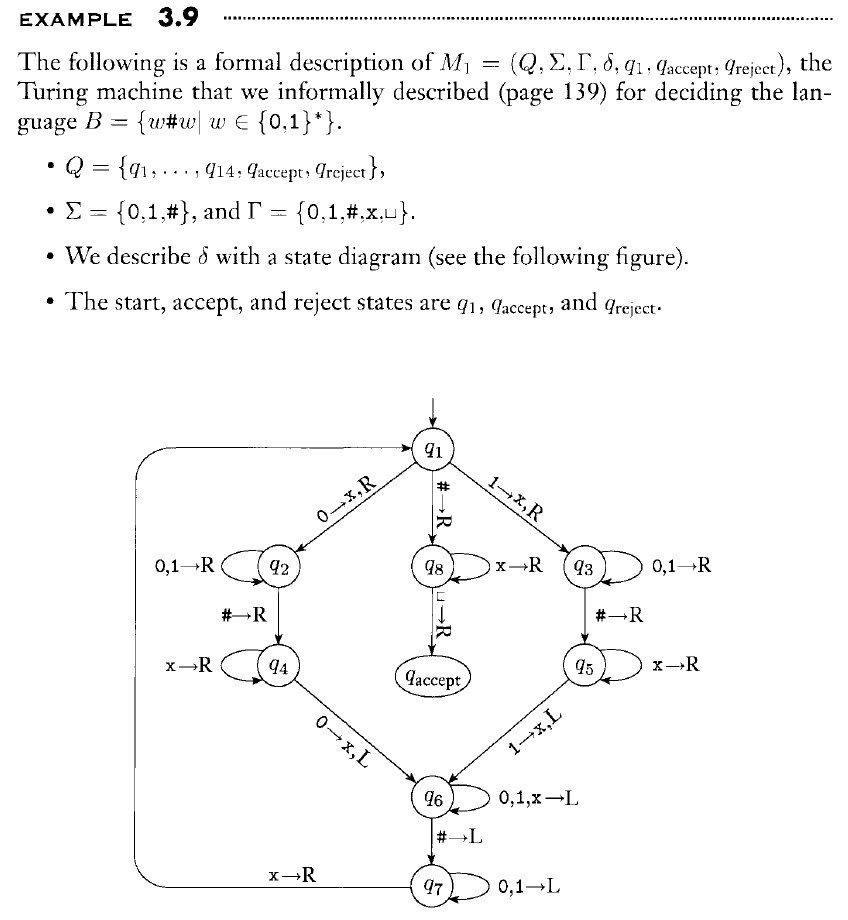
\includegraphics[scale=0.5]{./Cours2_Ex3_9.jpg}
    \end{figure}
  \end{center}

  Lorsque l'on est en $q_1$ et que l'on voit un 0, on peut écrire: $\delta(q_1, 0) = (q_2, x, R)$\\
  \begin{align*}
    \delta(q_2, 0) &= (q_2, 0, R)\\
    \delta(q_2, 1) &= (q_2, 1, R)
  \end{align*}
  Note: ''\textvisiblespace`` désigne le symbole ''blanc``, vide...

  \subsection{''Turing-decidabilité``}
    Un langage $L$ est ''Turing-decidable`` $\Leftrightarrow$ il existe une machine de Turing qui s'arrête sur toutes les entrées, comme si $L$ était la liste des états acceptés.\\
    Une machine de Turing qui s'arrête sur toutes les entrées (donc qui finit en un des deux états finaux $q_{\text{accepté}}$ ou $q_{\text{rej.}}$) est appelé ''Decider``.

  \subsection{''Turing-Recognizable``}
    Un langage $L$ est ''Turing-Recognizable`` $\Leftrightarrow$ il existe une machine de Turing telle que $L$ est une liste d'états d'entrée acceptables.  Parfois ici la machine ne s'arrête pas (et ces mots ne se donc pas dans le langage $L$).

  \subsection{Différence entre les deux}
    \textbf{Decidable}\\
    Si on prend l'entrée x.  Si il existe une machine de Turing tel que:
    \begin{itemize}
      \item si $x \in L$:  cela s'arrête sur $q_{\text{accepté}}$
      \item si $x \notin L$:  cela s'arrête sur $q_{\text{rejeté}}$
    \end{itemize}

    \textbf{Reconnaitre}\\
    Si on prend l'entrée x.  Si il existe une machine de Turing tel que:
    \begin{itemize}
      \item si $x \in L$:  cela s'arrête sur $q_{\text{accepté}}$
      \item si $x \notin L$:  cela s'arrête sur $q_{\text{rejeté}}$ OU il ne s'arrête jamais.
    \end{itemize}
    Par définition, les langages qui sont décidable, sont des langages que l'on peut ''reconnaitre``.

  \subsection{Variantes des machines de Turing}
    Livre 3.2 (page 148)

    \subsubsection{Multitape Turing machine}
      Si l'on a 3 rubans (de manière générale $K$ rubans), on pourrait donc écrire de manière mathématique
      $$\delta : Q \times \Gamma^{k} \rightarrow Q \times \Gamma^K \times \{L, R, S\}^K$$
      Où $\{L, R, S\}$ correspond (respectivement) à gauche (left), droite (right), rester (stay).\\
      \textbf{Exemple: } $\delta(q, (a, b, c)) \rightarrow (q', (a, b, d), (L, R, S))$\\
      \textbf{Théorème 3.13:} Chaque multitape Turing machine a un équivalent (single-tape) en Turing Machine.

    \subsubsection{Simuler du Multitape sur une simple Turing Machine}
      L'idée est de ''simuler`` les ''k tapes`` sur une seule en se déplaçant. Pour ce faire, on augmente l'alphabet $\Gamma$ avec ''\#`` et le symbole $\dot{x}$ pour chaque $x \in \Gamma$ représentant les têtes.\\
      Ici on ne fait pas attention à la complexité, l'efficacité.  C'est évidemment plus lourd de tout mettre sur un ruban mais l'important c'est que ça soit possible.

    \subsubsection{Machine de Turing non déterministe}
      $$\delta : Q \times \Gamma \rightarrow \mathcal P (Q \times \Gamma \times \{L, R\})$$
      On va donc avoir des ''branches`` d’exécution.  Quand l'entrée est acceptée, cela signifie qu'il existe une branche menant à $q_{\text{accepté}}$

  \subsection{Computation tree (arbre d'exécution)}
    \textbf{Théorème 3.16} Chaque NTP a un équivalent (D)TM (qui reconnait donc le même langage).\\
    Il y a plusieurs moyen de parcourir cet arbre: parcours en profondeur, parcours par niveau, parcours en largeur.  C'est ce dernier algorithme qui sera privilégié.  Pour faire cela avec un TM, on va utiliser un 3-Tape (3 rubans) Turing machine déterministe.\\
    On aura donc 3 rubans avec: l'entrée, la simulation et l'adresse.  En simulant cela, on va pouvoir voir si on arrive sur un statut accepté.

\end{document}
